\documentclass[tikz,border=5]{standalone}
\usetikzlibrary{fit,positioning,arrows.meta}
\tikzset{neuron/.style={shape=circle, minimum size=1.25cm, 
  inner sep=0, draw, font=\small}, io/.style={neuron, fill=gray!20}}
\begin{document}
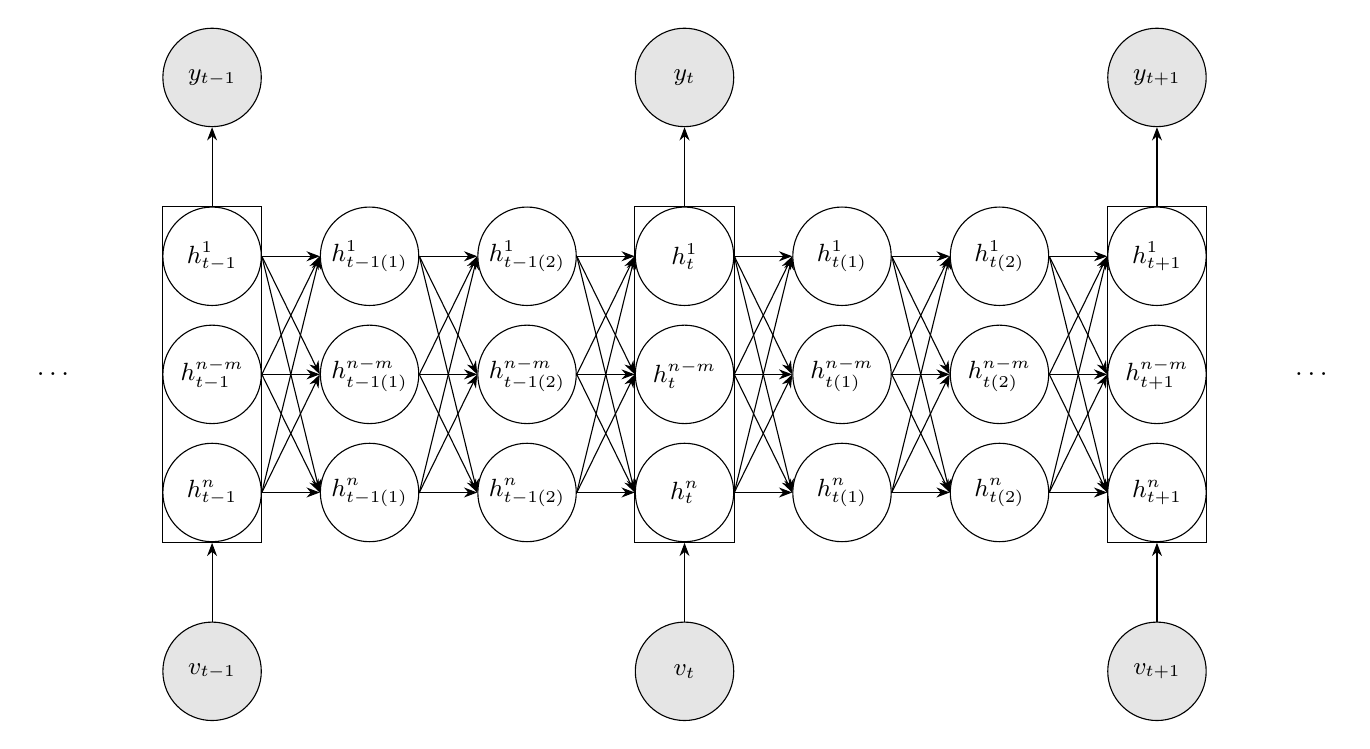
\begin{tikzpicture}[x=2cm, y=1.5cm, >=Stealth]
    \foreach \jlabel [count=\j, evaluate={\k=int(mod(\j-1,3)); \jj=int(\j-1);}]
    in {t-1, t-1(1), t-1(2), t, t(1), t(2), t+1}{
            \foreach \ilabel [count=\i] in {1, n-m, n}
            \node [neuron] at (\j, 1-\i) (h-\i-\j){$h_{\jlabel}^{\ilabel}$};
            \ifcase\k
                \node [fit=(h-1-\j) (h-3-\j), inner sep=0, draw] (b-\j) {};
                \node [io, above=of b-\j] (y-\j) {$y_{\jlabel}$};
                \node [io, below=of b-\j] (v-\j) {$v_{\jlabel}$};
                \draw [->] (v-\j) -- (b-\j);
                \draw [->] (b-\j) -- (y-\j);
            \fi
            \ifnum\j>1
                \foreach\i in {1, 2, 3}
                \foreach \ii in {1, 2, 3}
                \draw [->] (h-\i-\jj.east) -- (h-\ii-\j.west);
            \fi
        }
    \node [left=of h-2-1] {\ldots};
    \node [right=of h-2-7] {\ldots};
\end{tikzpicture}
\end{document}